\chapter{NumPy Basics: Arrays and Vectorized Computation}
NumPy, short for Numerical Python, is one of the most important foundational packages for numerical computing in Python. 

Here are some of the things you'll find in NumPy:
\begin{itemize}
    \item ndarray, an efficient multidimensional array providing fast array-oriented arithmetic operations and flexible broadcasting capabilities
    \item Mathematical functions for fast operations on entire arrays of data without having to write loops
    \item Tools for reading/writing array data to disk and working with memory-mapped files
    \item Linear algebra, random number generation, and Fourier transform capabilities
    \item A C API for connecting NumPy with libraries written in C, C++, or FORTRAN
\end{itemize}

For most data analysis applications, the main areas of functionality I'll focus on are:

\begin{itemize}
    \item Fast array-based operations for data munging and cleaning, subsetting and filtering, transformation, and any other kind of computation
    \item Common array algorithms like sorting, unique, and set operations
    \item Efficient descriptive statistics and aggregating/summarizing data
    \item Data alignment and relational data manipulations for merging and joining heterogeneous datasets
    \item Expressing conditional logic as array expressions instead of loops with \verb|if-elif-else| branches
    \item Group-wise data manipulations (aggregation, transformation, and function application)
\end{itemize}

One of the reasons NumPy is so important for numerical computations in Python is because it is designed for efficiency on large arrays of data. There are a number of reasons for this:
\begin{itemize}
    \item NumPy internally stores data in a contiguous block of memory, independent of other built-in Python objects. NumPy's library of algorithms written in the C language can operate on this memory without any type checking or other overhead. NumPy arrays also use much less memory than built-in Python sequences.
    \item NumPy operations perform complex computations on entire arrays without the need for Python for loops, which can be slow for large sequences. NumPy is faster than regular Python code because its C-based algorithms avoid overhead present with regular interpreted Python code.
\end{itemize}

\begin{pyc}
import numpy as np
my_arr = np.arange(1_000_000)
my_list = list(range(1_000_000))

%timeit my_arr2 = my_arr * 2
%timeit my_list2 = [x * 2 for x in my_list]
\end{pyc}
\section{The NumPy ndarray: A Multidimensional Array Object}
One of the key features of NumPy is its N-dimensional array object, or ndarray, which is a fast, flexible container for large datasets in Python. Arrays enable you to perform mathematical operations on whole blocks of data using similar syntax to the equivalent operations between scalar elements.
\begin{pyc}
import numpy as np

data = np.array([[1.5, -.1, 3], [0, -3, 6.5]])
data * 10
data + data
\end{pyc}

\notes{
    In this chapter and throughout the book, I use the standard NumPy convention of always using import numpy as np. It would be possible to put from numpy import * in your code to avoid having to write np., but I advise against making a habit of this. The numpy namespace is large and contains a number of functions whose names conflict with built-in Python functions (like min and max). Following standard conventions like these is almost always a good idea.
}

An ndarray is a generic multidimensional container for homogeneous data; that is, all of the elements must be the same type. Every array has a \verb|shape|, a tuple indicating the size of each dimension, and a \verb|dtype|, an object describing the \emph{data type} of the array:

\notes{
    Whenever you see “array”, “NumPy array,” or “ndarray”, in most cases they all refer to the ndarray object.
}
\subsection{Creating ndarrays}
The easiest way to create an array is to use the \verb|array| function. This accepts any sequence-like object (including other arrays) and produces a new NumPy array containing the passed data.
\begin{pyc}
data1 = [6, 7.5, 8, 0, 1]
arr1 = np.array(data1)
arr1
\end{pyc}

Nested sequences, like a list of equal-length lists, will be converted into a multidimensional array:
\begin{pyc}
data2 = [[1, 2, 3, 4], [5, 6, 7, 8]]
arr2 = np.array(data2)
arr2
\end{pyc}

Unless explicitly specified (discussed in \autoref{Data Types for ndarrays}), numpy.array tries to infer a good data type for the array that it creates. The data type is stored in a special dtype metadata object.
\begin{pyc}
print(arr1.dtype) # float64
print(arr2.dtype) # int32 
\end{pyc}

In addition to numpy.array, there are a number of other functions for creating new arrays. To create a higher dimensional array with these methods, pass a tuple for the shape:
\begin{pyc}
np.zeros(10)
np.zeros((3, 6))
np.empty((1, 2, 3))    
\end{pyc}

\warning{
    It's not safe to assume that numpy.empty will return an array of all zeros. This function returns uninitialized memory and thus may contain nonzero “garbage” values. You should use this function only if you intend to populate(填充) the new array with data.
}

\verb|numpy.arange| is an array-valued version of the built-in Python range function:
\begin{pyc}
np.arange(15)
# array([ 0,  1,  2,  3,  4,  5,  6,  7,  8,  9, 10, 11, 12, 13, 14])
\end{pyc}

See \autoref{Some important NumPy array creation functions} for a short list of standard array creation functions. Since NumPy is focused on numerical computing, the data type, if not specified, will in many cases be float64 (floating point).

\begin{table}
    \caption{Some important NumPy array creation functions}
    \label{Some important NumPy array creation functions}
    \begin{tabularx}{\textwidth}{lX}
        \hline
        Function                        & Description                                                                                                                                                                                          \\
        \hline
        \verb|array|                    & Convert input data (list, tuple, array, or other sequence type) to an ndarray either by inferring a data
        type or explicitly specifying a data type; copies the input data by default                                                                                                                                                            \\
        \verb|asarray|                  & Convert input to ndarray, but do not copy if the input is already an ndarray                                                                                                                         \\
        \verb|arange|                   & Like the built-in range but returns an ndarray instead of a list                                                                                                                                     \\
        \verb|ones|, \verb|ones_like|   & Produce an array of all 1s with the given shape and data type; \verb|ones_like| takes another array and produces a ones array of the same shape and data type                                        \\
        \verb|zeros|, \verb|zeros_like| & Like \verb|ones| and \verb|ones_like| but producing arrays of 0s instead                                                                                                                             \\
        \verb|empty|, \verb|empty_like| & Create new arrays by allocating new memory, but do not populate with any values like \verb|ones| and \verb|zeros|                                                                                    \\
        \verb|full|, \verb|full_like|   & Produce an array of the given shape and data type with all values set to the indicated “fill value”; \verb|full_like| takes another array and produces a filled array of the same shape and data type \\
        \verb|eye|, \verb|identity|     & Create a square $N \times N$ identity matrix (1s on the diagonal and 0s elsewhere)                                                                                                                   \\
        \hline
    \end{tabularx}
\end{table}
\subsection{Data Types for ndarrays\label{Data Types for ndarrays}}
The data type or dtype is a special object containing the information (or metadata, data about data) the ndarray needs to interpret a chunk of memory as a particular type of data:
\begin{pyc}
arr1 = np.array([1, 2, 3], dtype=np.float64)
arr2 = np.array([1, 2, 3], dtype=np.int32)
print(arr1.dtype) # float64
print(arr2.dtype) # int32
\end{pyc}
\notes{
    Don't worry about memorizing the NumPy data types, especially if you're a new user. It's often only necessary to care about the general kind of data you're dealing with, whether floating point, complex, integer, Boolean, string, or general Python object. When you need more control over how data is stored in memory and on disk, especially large datasets, it is good to know that you have control over the storage type.
}
See \autoref{NumPy data types} for a full listing of NumPy's supported data types.
\begin{table}
    \caption{NumPy data types}
    \label{NumPy data types}
    \begin{tabularx}{\textwidth}{llX}
        \hline
        Type                                                   & Type code                         & Description                                                                                                                 \\
        \hline
        \verb|int8|, \verb|uint8|                              & \verb|i1|, \verb|u1|              & Signed and unsigned 8-bit (1 byte) integer types                                                                            \\
        \verb|int16|, \verb|uint16|                            & \verb|i2|, \verb|u2|              & Signed and unsigned 16-bit integer types                                                                                    \\
        \verb|int32|, \verb|uint32|                            & \verb|i4|, \verb|u4|              & Signed and unsigned 32-bit integer types                                                                                    \\
        \verb|int64|, \verb|uint64|                            & \verb|i8|, \verb|u8|              & Signed and unsigned 64-bit integer types                                                                                    \\
        \verb|float16|                                         & \verb|f2|                         & Half-precision floating point                                                                                               \\
        \verb|float32|                                         & \verb|f4| or \verb|f|             & Standard single-precision floating point; compatible with C float                                                           \\
        \verb|float64|                                         & \verb|f8| or \verb|d|             & Standard double-precision floating point; compatible with C double and Python float object                                  \\
        \verb|float128|                                        & \verb|f16| or \verb|g|            & Extended-precision floating point                                                                                           \\
        \verb|complex64|, \verb|complex128|, \verb|complex256| & \verb|c8|, \verb|c16|, \verb|c32| & Complex numbers represented by two 32, 64, or 128 floats, respectively                                                      \\
        \verb|bool|                                            & \verb|?|                          & Boolean type storing True and False values                                                                                  \\
        \verb|object|                                          & \verb|O|                          & Python object type; a value can be any Python object                                                                        \\
        \verb|string_|                                         & \verb|S|                          & Fixed-length ASCII string type (1 byte per character); for example, to create astring data type with length 10, use 'S10'   \\                                                                                                                          
        \verb|unicode_|                                        & \verb|U|                          & Fixed-length Unicode type (number of bytes platform specific); same specification semantics as \verb|string_| (e.g., 'U10') \\
        \hline
    \end{tabularx}
\end{table}

\notes{There are both signed and unsigned integer types, and many readers
will not be familiar with this terminology. A signed integer can
represent both positive and negative integers, while an unsigned
integer can only represent nonnegative integers. For example, int8
(signed 8-bit integer) can represent integers from -128 to 127
(inclusive), while uint8 (unsigned 8-bit integer) can represent 0
through 255.}

You can explicitly convert or cast an array from one data type to another using ndarray's \verb|astype| method:
\begin{pyc}
arr = np.array([1, 2, 3, 4, 5])
print(arr) # [1 2 3 4 5]
print(arr.dtype) # int32
float_arr = arr.astype(np.float64)
print(float_arr) # [1. 2. 3. 4. 5.]
print(float_arr.dtype) # float64
\end{pyc}

If I cast some floating-point numbers to be of integer data type, the decimal part will be truncated:
\begin{pyc}
arr = np.array([3.7, -1.2, -2.6, 0.5, 12.9, 10.1])
print(arr)
arr.astype(np.int32)
# array([ 3, -1, -2,  0, 12, 10])
\end{pyc}

If you have an array of strings representing numbers, you can use astype to convert them to numeric form:
\begin{pyc}
numeric_strings = np.array(['1.25', '-9.6', '42'], dtype=np.string_)
numeric_strings.astype(float)
# array([ 1.25, -9.6 , 42.  ])
\end{pyc}

\warning{
    Be cautious when using the numpy.string\_ type, as string data in NumPy is fixed size and may truncate input without warning. pandas has more intuitive out-of-the-box behavior on non-numeric data.
}

If casting were to fail for some reason (like a string that cannot be converted to float64), a ValueError will be raised. Before, I was a bit lazy and wrote float instead of np.float64; NumPy aliases the Python types to its own equivalent data types.

You can also use another array's dtype attribute:
\begin{pyc}
int_array = np.arange(10)

calibers = np.array([.22, .270, .357, .44, .50], dtype=np.float64)
int_array.astype(calibers.dtype)
# array([0., 1., 2., 3., 4., 5., 6., 7., 8., 9.])
\end{pyc}

There are shorthand type code strings you can also use to refer to a dtype.

\notes{
    Calling astype always creates a new array (a copy of the data), even if the new data type is the same as the old data type.
}

\subsection{Arithmetic with NumPy Arrays}
Arrays are important because they enable you to express batch operations on data  without writing any for loops. NumPy users call this \emph{vectorization}.
\begin{itemize}
    \item Any arithmetic operations between equal-size arrays apply the operation element-wise
    \item Arithmetic operations with scalars propagate the scalar argument to each element in the array
    \item Comparisons between arrays of the same size yield Boolean arrays
\end{itemize}
\begin{pyc}
arr = np.array([[1., 2., 3.], [4., 5., 6.]])
arr * arr
arr - arr

1 / arr
arr ** 2

arr2 = np.array([[0., 4., 1.], [7., 2., 12.]])
arr2 > arr
\end{pyc}
Evaluating operations between differently sized arrays is called broadcasting and will be discussed in more detail in \nameref{Appendix A}.
\subsection{Basic Indexing and Slicing}
NumPy array indexing is a deep topic, as there are many ways you may want to select a subset of your data or individual elements.

\begin{pyc}
arr = np.arange(10)
arr[5]
# 5

arr[5: 8]
# array([5, 6, 7])

arr[5: 8] = 12
arr
# array([ 0,  1,  2,  3,  4, 12, 12, 12,  8,  9])
\end{pyc}
\notes{
    An important first distinction from Python's built-in lists is that \textbf{array slices are views on the original array}. This means that the data is not copied, and any modifications to the view will be reflected in the source array. 
}

\begin{pyc}
arr_slice = arr[5: 8]
arr_slice
# array([12, 12, 12])
arr_slice[1] = 123
arr
# array([  0,   1,   2,   3,   4,  12, 123,  12,   8,   9])

arr_slice[:] = 64
arr
# array([ 0,  1,  2,  3,  4, 64, 64, 64,  8,  9])
\end{pyc}
\paragraph{Pythonn内置的列表}
\begin{pyc}
a = list(range(10))
print(a)
# [0, 1, 2, 3, 4, 5, 6, 7, 8, 9]
b = a[2: 5]
# [2, 3, 4]
print(b)
b[1] = 1234
print(b)
# [2, 1234, 4]
print(a)
# [0, 1, 2, 3, 4, 5, 6, 7, 8, 9]
\end{pyc}

As NumPy has been designed to be able to work with very large arrays, you could imagine performance and memory problems if NumPy insisted on always copying data.

\warning{
    If you want a copy of a slice of an ndarray instead of a view, you will need to explicitly copy the array—for example, arr[5:8].copy(). As you will see, pandas works this way, too.
}

With higher dimensional arrays, you have many more options. In a two-dimensional
array, the elements at each index are no longer scalars but rather one-dimensional
arrays. Thus, individual elements can be accessed recursively. But that is a bit too much
work, so you can pass a comma-separated list of indices to select individual elements.

\begin{pyc}
arr2d = np.array([[1, 2, 3], [4, 5, 6], [7, 8, 9]])
arr2d[2]
# array([7, 8, 9])

# these are equivalent:
arr2d[0][2]
arr2d[0, 2]
\end{pyc}

See \autoref{Indexing elements in a NumPy array} for an illustration of indexing on a two-dimensional array. I find it helpful to think of axis 0 as the “rows” of the array and axis 1 as the “columns.”
\begin{figure}
    \centering
    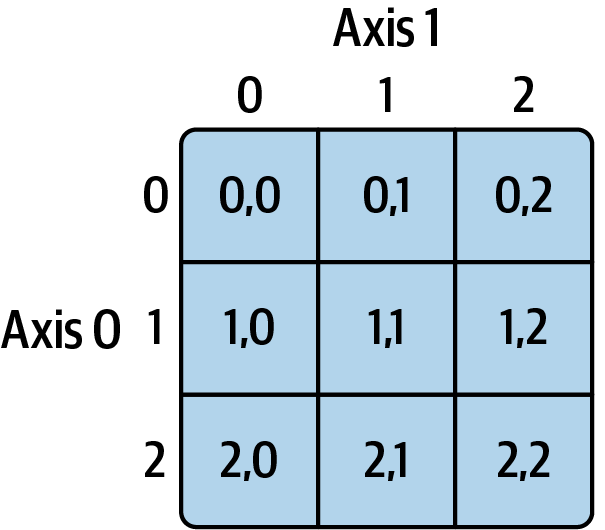
\includegraphics[width=.5\textwidth]{img/codes/Indexing elements in a NumPy array.png}
    \caption{Indexing elements in a NumPy array}
    \label{Indexing elements in a NumPy array}
\end{figure}

In multidimensional arrays, if you omit later indices, the returned object will be a
lower dimensional ndarray consisting of all the data along the higher dimensions. 

Note that in all of these cases where subsections of the array have been selected, the
returned arrays are views.

\warning{
    This multidimensional indexing syntax for NumPy arrays will not work with regular Python objects, such as lists of lists.
}
\subsubsection{Indexing with slices}
Like one-dimensional objects such as Python lists, ndarrays can be sliced with the
familiar syntax.

By mixing integer indexes and slices, you get lower dimensional slices.

\begin{figure}
    \centering
    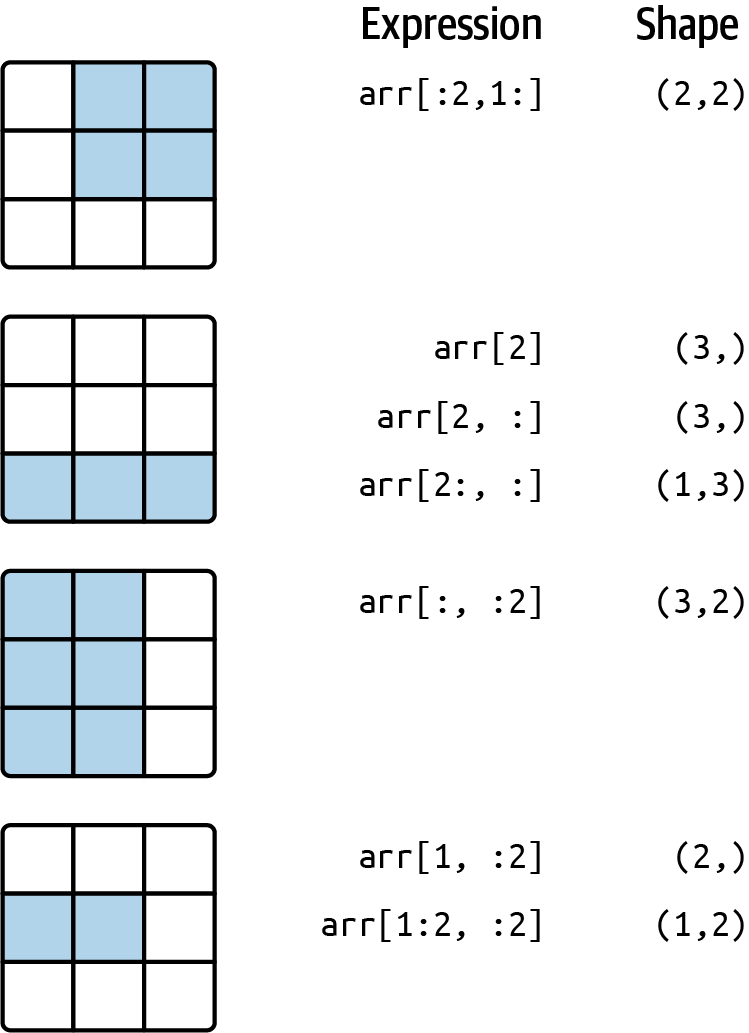
\includegraphics[width=.5\textwidth]{img/codes/Two-dimensional array slicing.png}
    \caption{Two-dimensional array slicing}
    \label{Two-dimensional array slicing}
\end{figure}

\begin{pyc}
lower_dim_slice = arr2d[1, :2]
lower_dim_slice.shape

arr2d[:2, 2]
arr2d[:, :1]

arr2d[:2, 1:] = 0
arr2d
\end{pyc}
\subsection{Boolean Indexing}
The Boolean array must be of the same length as the array axis it's indexing. You can even mix and match Boolean arrays with slices or integers (or sequences of integers).

\begin{pyc}
names = np.array(["Bob", "Joe", "Will", "Bob", "Will", "Joe", "Joe"])
print(names)
data = np.array([[4, 7], [0, 2], [-5, 6], [0, 0], [1, 2], [-12, 4], [3, 4]])
print(data)
print(names == "Bob")
print(data[names == "Bob"])
print(data[names == "Bob", 1:])
print(data[names == "Bob", 1])
\end{pyc}

\begin{itemize}
    \item To select everything but "Bob" you can either use != or negate the condition using $\sim$
    \item The $\sim$ operator can be useful when you want to invert a Boolean array referenced by a variable
    \item To select two of the three names to combine multiple Boolean conditions, use Boolean arithmetic operators like \verb|&| (and) and \textbar (or).
\end{itemize}

\begin{pyc}
names = np.array(["Bob", "Joe", "Will", "Bob", "Will", "Joe", "Joe"])
names
data = np.array([[4, 7], [0, 2], [-5, 6], [0, 0], [1, 2], [-12, 4], [3, 4]])
data
names == "Bob"
data[names == "Bob"]
data[names == "Bob", 1:]
data[names == "Bob", 1]

names != "Bob"
~(names == "Bob")
data[~(names == "Bob")]
cond = names == "Bob"
data[~cond]

mask = (names == "Bob") | (names == "Will")
data[mask]  
\end{pyc}

\textbf{Selecting data from an array by Boolean indexing and assigning the result to a new variable always creates a copy of the data}, even if the returned array is unchanged.

\warning{
    The Python keywords and and or do not work with Boolean arrays.
Use \& (and) and \textbar (or) instead.
}

\begin{itemize}
    \item Setting values with Boolean arrays works by substituting the value or values on the righthand side into the locations where the Boolean array's values are True.
    \item You can also set whole rows or columns using a one-dimensional Boolean array
\end{itemize}

\begin{pyc}
data[data < 0] = 0
data

data[names != "Joe"] = 7
data
\end{pyc}
\subsection{Fancy Indexing}
Fancy indexing is a term adopted by NumPy to describe indexing using integer arrays.
\begin{itemize}
    \item To select a subset of the rows in a particular order, you can simply pass a list or
    ndarray of integers specifying the desired order. Using negative indices selects rows from
    the end
    \item Passing multiple index arrays does something slightly different; it selects a one-dimensional array of elements corresponding to each tuple of indices.(返回的是一个一维的数组,这超乎了我的想象)
\end{itemize}

\begin{pyc}
arr = np.zeros((8, 4))
for i in range(8):
    arr[i] = i
arr

arr[[4, 3, 0, 6]]

arr[[-3, -5, -7]]

arr = np.arange(32).reshape((8, 4))
arr[[1, 5, 7, 2], [0, 3, 1, 2]]
\end{pyc}

To learn more about the reshape method, have a look at \nameref{Appendix A}. Here the elements (1, 0), (5, 3), (7, 1), and (2, 2) were selected. The result of fancy indexing with as many integer arrays as there are axes is always one-dimensional.

如果你想要返回一个二维的数组,你写的索引位置应该也得是一个矩形数组,下面是一种写法:
\begin{pyc}
arr[[1, 5, 7, 2]][:, [0, 3, 1, 2]]
\end{pyc}

Keep in mind that fancy indexing, unlike slicing, always copies the data into a new array when assigning the result to a new variable. If you assign values with fancy indexing, the indexed values will be modified.

\begin{pyc}
a = arr[[1, 5, 7, 2], [0, 3, 1, 2]]
a[0] = 10000
print(a)
print(arr)
\end{pyc}
\subsection{Transposing Arrays and Swapping Axes}
Transposing is a special form of reshaping that similarly returns a view on the underlying data without copying anything.
\begin{itemize}
    \item Arrays have the transpose method and the special T attribute. When doing matrix computations, you may do this very often. The @ infix operator is another way to do matrix multiplication.
    \item Simple transposing with .T is a special case of swapping axes. ndarray has the method \verb|swapaxes|, which takes a pair of axis numbers and switches the indicated axes to rearrange the data. 只返回源数据的视图,不会复制数据。
    \item 对于高维数组,transpose需要得到一个由轴编号组成的元组才能对这些轴进行转置(费脑子,不要用图像理解)。用代数的方法理解,原本$x_{103}=11$,轴变换后$x_{310}=11$或者$(1, 0, 3)=x_{103}$,变换后$(3, 1, 0)=x_{103}$。
\end{itemize}
\begin{pyc}
arr = np.arange(15).reshape((3, 5))
arr.T

arr = np.array([[0, 1, 0], [1, 2, -2], [6, 3, 2], [-1, 0, -1], [1, 0, 1]])
np.dot(arr.T, arr)
arr.T @ arr

arr.swapaxes(0, 1)

arr = np.arange(16).reshape((2, 2, 4))
arr.transpose((2, 0, 1))
\end{pyc}
\section{Pseudorandom Number Generation(伪随机数生成)}
\begin{enumerate}
    \item The \verb|numpy.random| module supplements the built-in Python random module with functions for efficiently generating whole arrays of sample values from many kinds of probability distributions. 
    \item Python's built-in \verb|random| module, by contrast, samples only one value at a time. As you can see from this benchmark, \verb|numpy.random| is well over an order of magnitude faster for generating very large samples(要快一个数量级).
    \item These random numbers are not truly random (rather, pseudorandom) but instead are generated by a configurable random number generator that determines deterministically what values are created. Functions like \verb|numpy.random.standard_normal| use the numpy.random module's default random number generator, but your code can be configured to use an explicit generator.
    \item The seed argument is what determines the initial state of the generator, and the state changes each time the rng object is used to generate data. The generator object rng is also isolated from other code which might use the numpy.random module. 和随机数种子不一样,每次还是会产生不同的随机数,仅仅是修改一些随机数生成器的配置文件。
\end{enumerate}

\begin{pyc}
samples = np.random.standard_normal(size=(4, 4))
samples

from random import normalvariate
N = 1_000_000

%timeit samples = [normalvariate(0, 1) for _ in range(N)]

%timeit np.random.standard_normal(N)

rng = np.random.default_rng(seed=42)
data = rng.standard_normal((2, 3))

type(rng)
# numpy.random._generator.Generator
\end{pyc}

See \autoref{NumPy random number generator methods} for a partial list of methods available on random generator objects like \verb|rng|(random number generator).

\begin{table}
    \caption{NumPy random number generator methods}
    \label{NumPy random number generator methods}
    \begin{tabularx}{\textwidth}{lX}
        \hline
        Methods                & Description                                                                  \\
        \hline
        \verb|permutation|     & Return a random permutation of a sequence, or return a permuted range        \\
        \verb|shuffle|         & Randomly permute a sequence in place(没有任何的返回None,需要接收一个可迭代对象,这个对象将被随机打乱)                                         \\
        \verb|uniform|         & Draw samples from a uniform distribution                                     \\
        \verb|randint|         & Draw random integers from a given low-to-high range                          \\
        \verb|standard_normal| & Draw samples from a normal distribution with mean 0 and standard deviation 1 \\
        \verb|binomial|        & Draw samples from a binomial distribution                                    \\
        \verb|normal|          & Draw samples from a normal (Gaussian) distribution                           \\
        \verb|beta|            & Draw samples from a \href{https://numpy.org/doc/stable/reference/random/generated/numpy.random.beta.html}{beta distribution}                                        \\                                    
        \verb|chisquare|       & Draw samples from a \href{https://numpy.org/doc/stable/reference/random/generated/numpy.random.chisquare.html}{chi-square distribution}                                  \\
        \verb|gamma|           & Draw samples from a \href{https://numpy.org/doc/stable/reference/random/generated/numpy.random.gamma.html}{gamma distribution}                                       \\
        \hline
    \end{tabularx}
\end{table}
\section{Universal Functions: Fast Element-Wise Array Functions}
A universal function, or \emph{ufunc}, is a function that performs element-wise operations
on data in ndarrays.
\begin{enumerate}
    \item Many ufuncs are simple element-wise transformations, like \verb|numpy.sqrt| or \verb|numpy.exp|. These are referred to as \emph{unary}(一元的) ufuncs.
    \item Others, such as \verb|numpy.add| or \verb|numpy.maximum|, take two arrays (thus, binary ufuncs) and return a single array as the result.
    \item While not common, a ufunc can return multiple arrays. \verb|numpy.modf| is one example: a vectorized version of the built-in Python \verb|math.modf|, it returns the fractional and integral parts of a floating-point array
    \item Ufuncs accept an optional out argument that allows them to assign their results into an existing array rather than create a new one
\end{enumerate}
\begin{pyc}
arr = np.arange(10)
np.sqrt(arr)
np.exp(arr)

x = rng.standard_normal(8)
y = rng.standard_normal(8)

np.maximum(x, y)

arr = rng.standard_normal(7) * 5
remainder, whole_part = np.modf(arr)
remainder
whole_part

arr
# 7 * 1
print(arr)
out = np.zeros_like(arr)
out = np.add(arr, 1)

np.add(arr, 1, out=out)
out
\end{pyc}

See \autoref{Some unary universal functions} and \autoref{Some unary universal functions} for a listing of some of NumPy's ufuncs. New ufuncs continue to be added to NumPy, so consulting the online NumPy documentation is the best way to get a comprehensive listing and stay up to date.

\begin{table}
    \caption{Some unary universal functions}
    \label{Some unary universal functions}
    \begin{tabularx}{\textwidth}{lX}
        \hline
        Function               & Description                                                                                                 \\
        \hline
        \verb|abs, fabs|       & Compute the absolute value element-wise for integer, floating-point, or complex values                      \\
        \verb|sqrt|            & Compute the square root of each element (equivalent to arr ** 0.5)                                          \\
        \verb|square|          & Compute the square of each element (equivalent to arr ** 2)                                                 \\
        \verb|exp|             & Compute the exponent $e^x$ of each element                                                                  \\
        \verb|log, log10|      & Natural logarithm (base e), log base 10, log base 2, and log(1 + x), respectively                           \\
        \verb|log2, log1p|     &                                                                                                             \\
        \verb|sign|            & Compute the sign of each element: 1 (positive), 0 (zero), or –1 (negative)                                  \\
        \verb|ceil|            & Compute the ceiling of each element (i.e., the smallest integer greater than or equal to that number)       \\
        \verb|floor|           & Compute the floor of each element (i.e., the largest integer less than or equal to each element)            \\
        \verb|rint|            & Round elements to the nearest integer, preserving the dtype                                                 \\
        \verb|modf|            & Return fractional and integral parts of array as separate arrays                                            \\
        \verb|isnan|           & Return Boolean array indicating whether each value is NaN (Not a Number)                                    \\
        \verb|isfinite, isinf| & Return Boolean array indicating whether each element is finite (non-inf, non-NaN) or infinite, respectively \\
        \verb|cos, cosh, sin|  & Regular and hyperbolic trigonometric functions                                                              \\
        \verb|sinh, tan, tanh| &                                                                                                             \\
        \verb|arccos, arccosh| & Inverse trigonometric functions                                                                             \\
        \verb|arcsin, arcsinh| &                                                                                                             \\
        \verb|arctan, arctanh| &                                                                                                             \\
        \verb|logical_not|     & Compute truth value of not x element-wise (equivalent to \verb|~arr|)                                       \\
        \hline
    \end{tabularx}
\end{table}

\begin{table}
    \caption{Some unary universal functions}
    \label{Some binary universal functions}
    \begin{tabularx}{\textwidth}{lX}
        \hline
        Function                    & Description                                                                                                   \\
        \hline
        \verb|add|                  & Add corresponding elements in arrays                                                                          \\
        \verb|subtract|             & Subtract elements in second array from first array                                                            \\
        \verb|multiply|             & Multiply array elements                                                                                       \\
        \verb|divide, floor_divide| & Divide or floor divide (truncating the remainder)                                                             \\
        \verb|power|                & Raise elements in first array to powers indicated in second array                                             \\
        \verb|maximum, fmax|        & Element-wise maximum; fmax ignores NaN                                                                        \\
        \verb|minimum, fmin|        & Element-wise minimum; fmin ignores NaN                                                                        \\
        \verb|mod|                  & Element-wise modulus (remainder of division)                                                                  \\
        \verb|copysign|             & Copy sign of values in second argument to values in first argument                                            \\
        \verb|greater, greater_equal, less|,             & Perform element-wise comparison, yielding Boolean array (equivalent to infix operators$>, >=, <, <=, ==, !=$) \\
        \verb|less_equal, equal|,   &                                                                                                               \\
        \verb|not_equal|            &                                                                                                               \\
        \verb|logical_and|          & Compute element-wise truth value of AND ( \& ) logical operation                                              \\
        \verb|logical_or|           & Compute element-wise truth value of OR (\textbar) logical operation                                           \\
        \verb|logical_xor|          & Compute element-wise truth value of XOR (\^{}) logical operation                                              \\
        \hline
    \end{tabularx}
\end{table}

\section{Array-Oriented Programming with Arrays}
Using NumPy arrays enables you to express many kinds of data processing tasks as
concise array expressions that might otherwise require writing loops. This practice
of replacing explicit loops with array expressions is referred to by some people
as vectorization. In general, vectorized array operations will usually be significantly
faster than their pure Python equivalents, with the biggest impact in any kind of
numerical computations.

The numpy.meshgrid function takes two one-dimensional arrays and produces two two-dimensional matrices corresponding to all pairs of $(x, y)$ in the two arrays:

\begin{pyc}
points = np.arange(-5, 5, .01)
xs, ys = np.meshgrid(points, points)

z = np.sqrt(xs ** 2 + ys ** 2)

import matplotlib.pyplot as plt
plt.imshow(z, cmap=plt.cm.gray, extent=[-5, 5, -5, 5])
plt.colorbar()
plt.title('Image plot of $\sqrt{x^2 + y^2}$ for a grid of values')
save_fig("Plot of function evaluated on a grid")
\end{pyc}

\figures{Plot of function evaluated on a grid}

\notes{The term \emph{vectorization} is used to describe some other computer science concepts, but in this book I use it to describe operations on whole arrays of data at once rather than going value by value using a Python for loop.}

\subsection{Expressing Conditional Logic as Array Operations}
The \verb|numpy.where| function is a vectorized version of the ternary expression \verb|x if condition else y|.

\begin{pyc}
xarr = np.array([1.1, 1.2, 1.3, 1.4, 1.5])
yarr = np.array([2.1, 2.2, 2.3, 2.4, 2.5])
cond = np.array([True, False, True, True, False])
\end{pyc}
Suppose we wanted to take a value from xarr whenever the corresponding value in cond is True, and otherwise take the value from yarr.
\begin{pyc}
result = [(x if c else y) for x, y, c in zip(xarr, yarr, cond)]
result
# [1.1, 2.2, 1.3, 1.4, 2.5]
\end{pyc}

This has multiple problems. First, it will not be very fast for large arrays (because all the work is being done in interpreted Python code). Second, it will not work with multidimensional arrays. With numpy.where you can do this with a single function call:
\begin{pyc}
result = np.where(cond, xarr, yarr)
\end{pyc}

The second and third arguments to numpy.where don't need to be arrays; one or both of them can be scalars. A typical use of where in data analysis is to produce a new array of values based on another array. You can combine scalars and arrays when using numpy.where. 
\begin{pyc}
arr = rng.standard_normal((4, 4))
np.where(arr > 0, 2, -2)

np.where(arr > 0, 2, arr)
\end{pyc}

\subsection{Mathematical and Statistical Methods}
A set of mathematical functions that compute statistics about an entire array or about the data along an axis are accessible as methods of the array class. You can use aggregations (sometimes called reductions) like sum, mean, and std (standard deviation) either by calling the array instance method or using the top-level NumPy function. When you use the NumPy function, like numpy.sum, you have to pass the array you want to aggregate as the first argument.

\begin{enumerate}
    \item Functions like mean and sum take an optional axis argument that computes the statistic over the given axis, resulting in an array with one less dimension. \verb|arr.mean(axis=1)| means “compute mean across the columns,” where \verb|arr.sum(axis=0)| means “compute sum down the rows.” 
    \item Other methods like cumsum and cumprod do not aggregate, instead producing an array of the intermediate results. In multidimensional arrays, accumulation functions like cumsum return an array of the same size but with the partial aggregates computed along the indicated axis according to each lower dimensional slice.
\end{enumerate}

\begin{pyc}
arr = rng.standard_normal((5, 4))
arr.mean()
np.mean(arr)
arr.sum()

arr.mean(axis=1)
# compute mean across the columns
arr.mean(axis=0)
# compute sum down the rows

arr = np.array([0, 1, 2, 3, 4, 5, 6, 7])
arr.cumsum()

arr2d = np.arange(9).reshape(-1, 3)
arr2d.cumsum(axis=0)
arr2d.cumsum(axis=1)
\end{pyc}

See \autoref{Basic array statistical methods} for a full listing.

\begin{table}
    \caption{Basic array statistical methods}
    \label{Basic array statistical methods}
    \begin{tabularx}{\textwidth}{lX}
        \hline
        Methods        & Description                                                                          \\
        \hline
        \verb|sum|            & Sum of all the elements in the array or along an axis; zero-length arrays have sum 0 \\
        \verb|mean|           & Arithmetic mean; invalid (returns NaN) on zero-length arrays                         \\
        \verb|std, var|       & Standard deviation and variance, respectively                                        \\
        \verb|min, max|       & Minimum and maximum                                                                  \\
        \verb|argmin, argmax| & Indices of minimum and maximum elements, respectively                                \\
        \verb|cumsum|         & Cumulative sum of elements starting from 0                                           \\
        \verb|cumprod|        & Cumulative product of elements starting from 1                                       \\
        \hline
    \end{tabularx}
\end{table}

\subsection{Methods for Boolean Arrays}
\begin{enumerate}
    \item Boolean values are coerced to 1 (True) and 0 (False) in the preceding methods. 
    \item Two additional methods, any and all, are useful especially for Boolean arrays. any tests whether one or more values in an array is True(存在), while all checks if every value is True(任意).
    \item These methods also work with non-Boolean arrays, where nonzero elements are treated as True.
\end{enumerate}

\begin{pyc}
arr = rng.standard_normal(100)
(arr > 0).sum()
(arr < 0).sum()

bools = np.array([False, False, True, False])
bools.any()
# True
bools.all()
# False

arr = np.array([0, 1, 1, 2, 2, 4])
arr.any()
# True
arr.all()
# False
\end{pyc}
\subsection{Sorting}
\begin{enumerate}
    \item Like Python's built-in list type, NumPy arrays can be sorted in place with the sort method.
    \item You can sort each one-dimensional section of values in a multidimensional array in place along an axis by passing the axis number to sort.
    \item The top-level method numpy.sort returns a sorted copy of an array (like the Python built-in function sorted) instead of modifying the array in place. 
\end{enumerate}

\begin{pyc}
arr = rng.standard_normal(5)
arr.sort()
arr

arr2d = rng.standard_normal((5, 3))
arr2d
arr2d.sort(axis=0)
arr2d
arr2d.sort(axis=1)
arr2d

arr2 = np.arange(10)
np.random.shuffle(arr2)

sorted_arr = np.sort(arr2)
sorted_arr

(sorted_arr == arr2).all()
\end{pyc}


For more details on using NumPy's sorting methods, and more advanced techniques like indirect sorts, see \nameref{Appendix A}.
\subsection{Unique and Other Set Logic}
NumPy has some basic set operations for one-dimensional ndarrays.

\begin{enumerate}
    \item A commonly used one is numpy.unique, which returns the sorted unique values in an array. In many cases, the NumPy version is faster and returns a NumPy array rather than a
    Python list.    
    \item Another function, numpy.in1d, tests membership of the values in one array in another, returning a Boolean array
\end{enumerate}

\begin{pyc}
names = np.array(["Bob", "Will", "Joe", "Bob", "Will", "Joe", "Joe"])
np.unique(names)
# array(['Bob', 'Joe', 'Will'], dtype='<U4')

ints = np.array([3, 3, 3, 2, 2, 1, 1, 4, 4])
np.unique(ints)
# array([1, 2, 3, 4])

# Contrast numpy.unique with the pure Python alternative
sorted(set(names))
# ['Bob', 'Joe', 'Will']

values = np.array([6, 0, 0, 3, 2, 5, 6])
np.in1d(values, [2, 3, 6])
# array([ True, False, False,  True,  True, False,  True])
\end{pyc}

See \autoref{Array set operations} for a listing of array set operations in NumPy.

\begin{table}
    \caption{Array set operations}
    \label{Array set operations}
    \begin{tabularx}{\textwidth}{lX}
        \hline
        Methods                  & Description                                    \\
        \hline
        \verb|unique(x)|         & Compute the sorted, unique elements in x       \\
        \verb|intersect1d(x, y)| & Compute the sorted, common elements in x and y \\
        \verb|union1d(x, y)|     & Compute the sorted union of elements           \\
        \verb|unique(x)|         & Compute the sorted, unique elements in x       \\
        \verb|intersect1d(x, y)| & Compute the sorted, common elements in x and y \\
        \verb|union1d(x, y)|     & Compute the sorted union of elements           \\
        \hline
    \end{tabularx}
\end{table}
\section{File Input and Output with Arrays}
NumPy is able to save and load data to and from disk in some text or binary formats. If you prefer pandas and other tools for loading text or tabular data, see \autoref{Data Loading, Storage, and File Formats} for much more.

\begin{enumerate}
    \item \verb|numpy.save| and \verb|numpy.load| are the two workhorse functions for efficiently saving and loading array data on disk. Arrays are saved by default in an uncompressed raw binary format with file extension \verb|.npy|. If the file path does not already end in .npy, the extension will be appended. The array on disk can then be loaded with numpy.load
    \item You can save multiple arrays in an uncompressed archive using \verb|numpy.savez| and passing the arrays as keyword arguments
    \item When loading an .npz file, you get back a dictionary-like object that loads the individual arrays lazily
    \item If your data compresses well, you may wish to use \verb|numpy.savez_compressed| instead. 
\end{enumerate}

\begin{pyc}
arr = np.arange(10)

np.save("some_array", arr)
np.load("some_array.npy")

np.savez("array_archive.npz", a=arr, b=arr)
arch = np.load("array_archive.npz")
arch["b"]

np.savez_compressed("array_compressed.npz", a=arr, b=arr)
\end{pyc}
\section{Linear Algebra}
Linear algebra operations, like matrix multiplication,decompositions, determinants(行列式), and other square matrix math, are an important part of many array libraries.
\begin{enumerate}
    \item Multiplying two two-dimensional arrays with $*$ is an element-wise product, while matrix multiplications require using a function. Thus, there is a function \verb|dot|S, both an array method and a function in the numpy namespace, for matrix multiplication. \verb|x.dot(y)| is equivalent to \verb|np.dot(x, y)|.
    \item numpy.linalg has a standard set of matrix decompositions and things like inverse and determinant
\end{enumerate}

See \autoref{Commonly used linear algebra functions} for a list of some of the most commonly used linear algebra functions.

\begin{table}
    \caption{Commonly used linear algebra functions}
    \label{Commonly used linear algebra functions}
    \begin{tabularx}{\textwidth}{lX}
        \hline
        Functions    & Description                                                                                                                                                \\
        \hline
        \verb|diag|  & Return the diagonal (or off-diagonal) elements of a square matrix as a 1D array, or convert a 1D array into a square matrix with zeros on the off-diagonal \\
        \verb|dot|   & Matrix multiplication                                                                                                                                      \\
        \verb|trace| & Compute the sum of the diagonal elements                                                                                                                   \\
        \verb|det|   & Compute the matrix determinant                                                                                                                             \\
        \verb|eig|   & Compute the eigenvalues and eigenvectors of a square matrix                                                                                                \\
        \verb|inv|   & Compute the inverse of a square matrix                                                                                                                     \\
        \verb|pinv|  & Compute the \href{https://en.wikipedia.org/wiki/Moore-Penrose_inverse}{Moore-Penrose pseudoinverse} of a matrix                                                                                                        \\
        \verb|qr|    & Compute the \href{https://en.wikipedia.org/wiki/QR_decomposition}{QR decomposition}                                                                                                                               \\
        \verb|svd|   & Compute the \href{https://en.wikipedia.org/wiki/Singular_value_decomposition}{singular value decomposition} (SVD, 奇异值分解)                                                                                                             \\
        \verb|solve| & Solve the linear system $Ax = b$ for $x$, where $A$ is a square matrix                                                                                     \\
        \verb|lstsq| & Compute the least-squares solution to $Ax = b$                                                                                                             \\
        \hline
    \end{tabularx}
\end{table}

\section{Example: Random Walks}
The simulation of \href{https://en.wikipedia.org/wiki/Random_walk}{random walks} provides an illustrative application of utilizing array operations. 

\begin{enumerate}
    \item Here is a pure Python way to implement a single random walk with 1,000 steps using the built-in random module. You might make the observation that walk is the cumulative sum of the random steps and could be evaluated as an array expression.
    \item From this we can begin to extract statistics like the minimum and maximum value along the walk's trajectory. A more complicated statistic is the first crossing time, the step at which the random walk reaches a particular value.
    \item Note that using argmax here is not always efficient because it always makes a full scan of the array. 
\end{enumerate}

\begin{pyc}
import random
position = 0
walk = [position]
n_steps = 1_000
for _ in range(n_steps):
    step = 1 if random.randint(0, 1) else -1
    position += step
    walk.append(position)
plt.plot(walk)

n_steps = 1_000
rng = np.random.default_rng(seed=12345)
# integers can work with objects made from np.random.default_rng
draws = rng.integers(0, 2, size=n_steps)
steps = np.where(draws == 0, 1, -1)
walk = steps.cumsum()
walk.min()
walk.max()
plt.plot(walk)

(np.abs(walk) >= 10).argmax()
\end{pyc}

\figures{A simple random walk}

\subsection{Simulating Many Random Walks at Once}
\begin{pyc}
n_walks = 5_000
n_steps = 1_000

draws  = rng.integers(0, 2, size=(n_walks, n_steps))
steps = np.where(draws > 0, 1, -1)
walks = steps.cumsum(axis=1)

walks.max()
walks.min()

hits30 = (np.abs(walks) >= 30).any(axis=1)
hits30.sum()

crossing_time = (np.abs(walks[hits30]) >= 30).argmax(axis=1)

crossing_time

crossing_time.mean()
\end{pyc}
\notes{Keep in mind that this vectorized approach requires creating an array with $nwalks \times nsteps$ elements, which may use a large amount of memory for large simulations. If memory is more constrained, then a different approach will be required.}
\section{Conclusion}
While much of the rest of the book will focus on building data wrangling skills with pandas, we will continue to work in a similar array-based style. In Appendix A, we will dig deeper into NumPy features to help you further develop your array computing skills.